\input format.tex
\input defs.tex

%% begin presentation

\title{\large \bfseries Distributed Deep Q-Learning}

\author{Hao Yi Ong, Kevin Chavez, and Augustus Hong\\[3ex]
CME 323, Stanford University}

\date{June 3, 2015}

\begin{document}

\frame{
\thispagestyle{empty}
\titlepage
}

\section{Introduction}

\begin{frame}{Motivation}
  \begin{itemize}\itemsep=12pt
  
    \item long-standing challenge of reinforcement learning (RL)
    \vspace*{0.5em}
    \begin{itemize}
        \item control with high-dimensional sensory inputs (\eg, vision, speech)
        \item shift away from reliance on hand-crafted features
    \end{itemize}
    
    \item utilize breakthroughs in deep learning for RL \cite{M+:13,M+:15}
    \vspace*{0.5em}
    \begin{itemize}
        \item extract high-level features from raw sensory data
        \item learn better representations than handcrafted features with neural network architectures used in supervised and unsupervised learning
    \end{itemize}

    \item create fast learning algorithm
    \vspace*{0.5em}
    \begin{itemize}
        \item train efficiently with stochastic gradient descent (SGD)
        \item distribute training process to accelerate learning \cite{D+:12}
    \end{itemize}

  \end{itemize}
\end{frame}

\begin{frame}{Success with Atari games}
    \begin{figure}
        \centering
        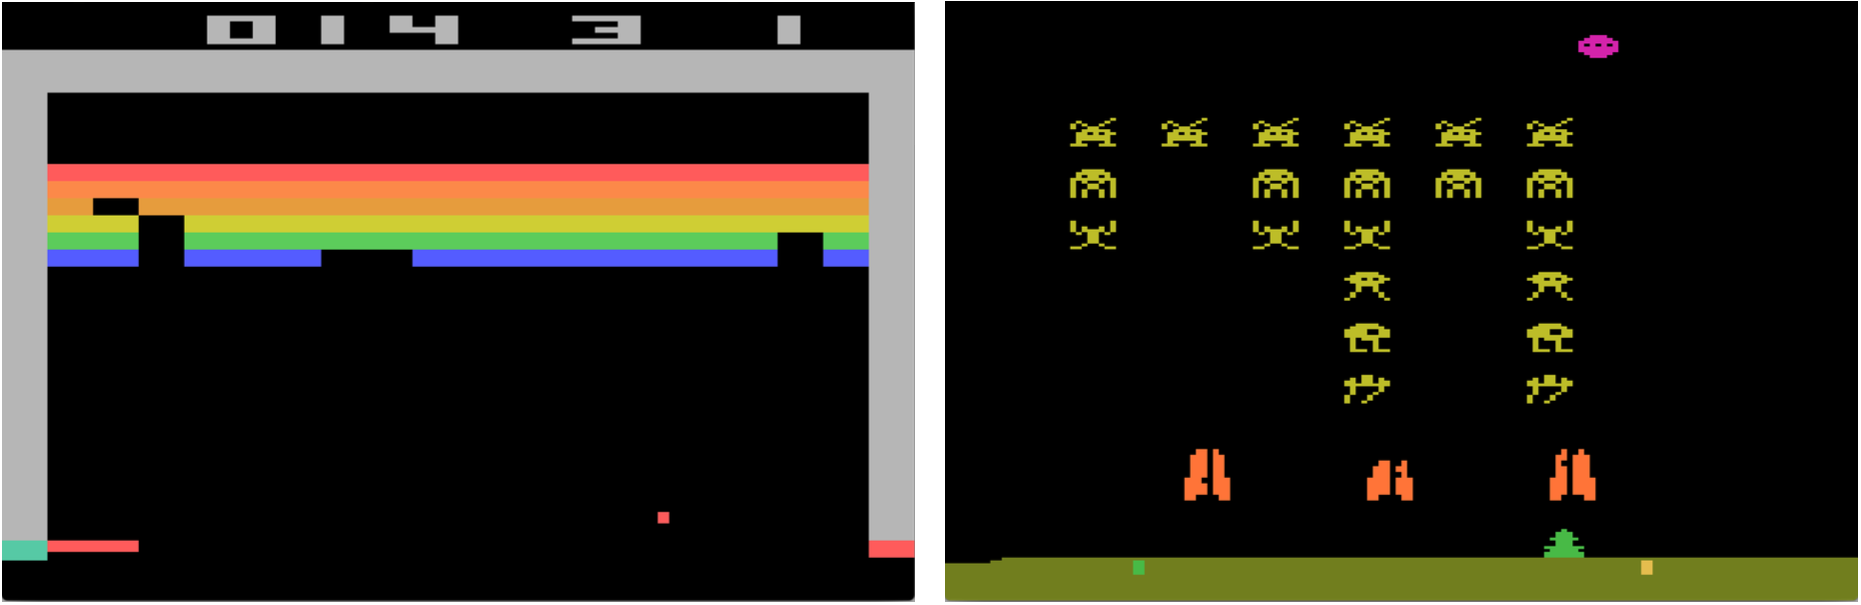
\includegraphics[width=0.8\textwidth]{atari-ex1.png}
    \end{figure}
    \begin{figure}
        \centering
        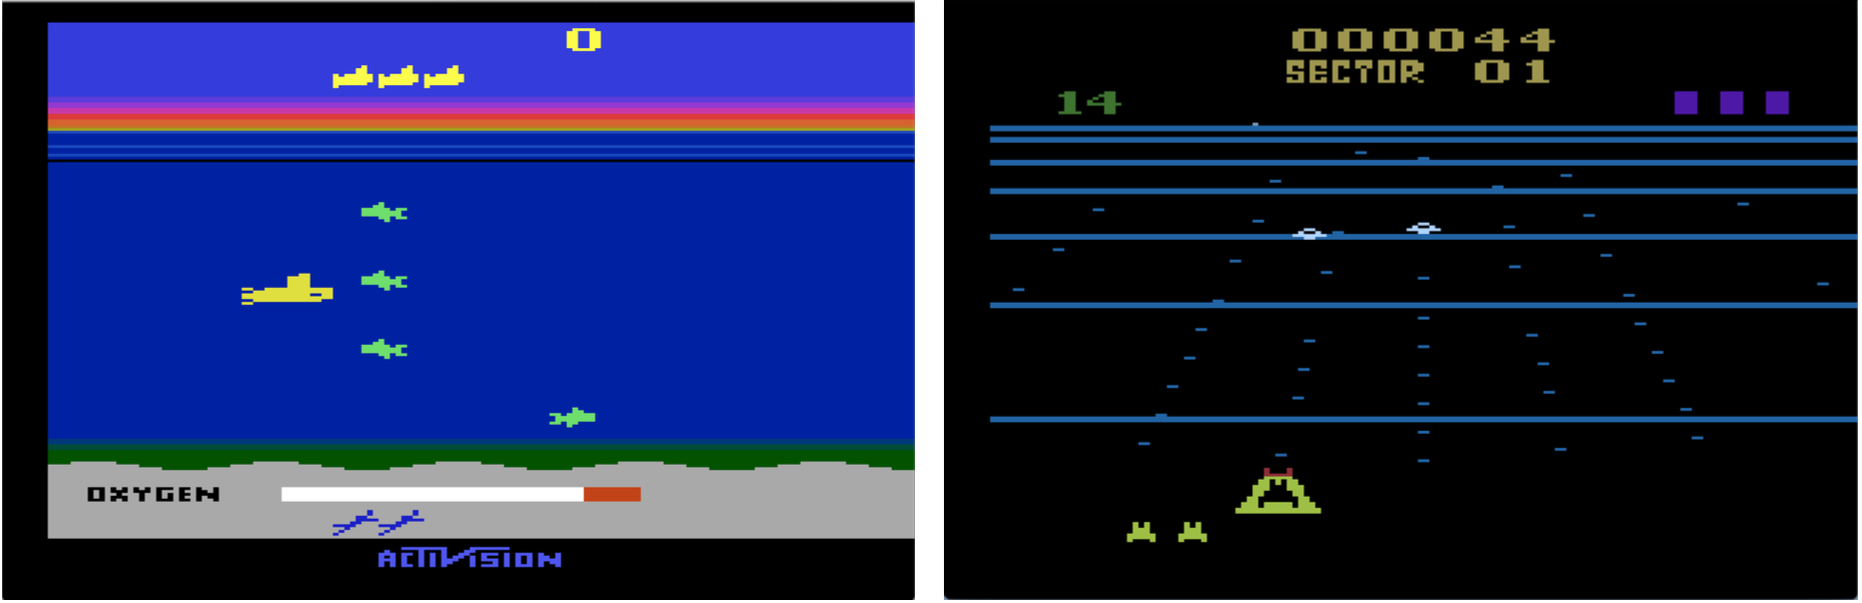
\includegraphics[width=0.8\textwidth]{atari-ex2.png}
    \end{figure}
\end{frame}

\begin{frame}{Goals}
    distributed deep RL algorithm
    \vspace*{0.5em}
    \begin{itemize}\itemsep=12pt
        
        \item robust neural network agent
        \vspace*{0.5em}
        \begin{itemize}
            \item must succeed in challenging test problems
        \end{itemize}

        \item control policies with high-dimensional sensory input
        \vspace*{0.5em}
        \begin{itemize}
            \item obtain better internal representations than handcrafted features
        \end{itemize}

        \item fast training algorithm
        \vspace*{0.5em}
        \begin{itemize}
            \item efficiently produce, use, and process training data
        \end{itemize}

    \end{itemize}
\end{frame}

\section{Mathematical formulation}

\begin{frame}{Playing games}
    \begin{figure}
        \centering
        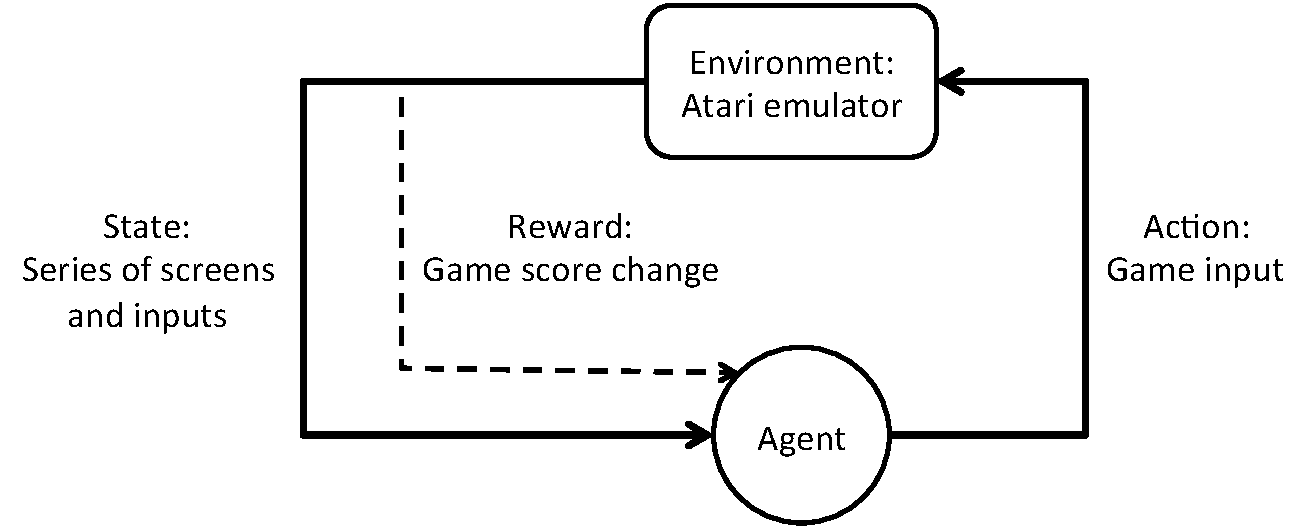
\includegraphics[width=0.8\textwidth]{background.pdf}
    \end{figure}
    \textbf{objective:} learned policy maximizes future rewards
    \[
        R_{t} = \sum_{t'=t}^{T} \gamma^{t'-t}r_{t'},
    \]
    \begin{itemize}
        \item discount factor $\gamma$
        \item reward change at time $t'$ $r_{t'}$
    \end{itemize}
\end{frame}

\begin{frame}{State-action value function}
    \begin{itemize}\itemsep=12pt
        
        \item basic idea behind RL is to estimate
        \[
            Q^{\star}\left(s, a\right) = 
            \max_{\pi}\Expect\left[R_{t} \mid s_{t} = s, a_{t} = a, \pi \right],
        \]
        where $\pi$ maps states to actions (or distributions over actions)

        \item optimal value function obeys Bellman equation
        \[
            Q^{\star}\left(s,a\right) = 
            \Expect_{s' \sim \mathcal{E}} \left[r + \gamma \max_{a'}Q^{\star}\left(s',a'\right)\mid s, a \right],
        \]
        where $\mathcal{E}$ is the MDP environment

    \end{itemize}
\end{frame}

\begin{frame}{Q-network}
    \begin{itemize}\itemsep=12pt

        \item trained by minimizing a sequence of loss functions
        \[
            L^{(i)}\left(\theta^{(i)}\right) =
            \Expect_{s,a \sim \rho\left(\cdot\right)}
            \left[\left(y^{(i)} - Q\left(s,a;\theta^{(i)}\right)\right)^{2}\right],
        \]
        with
        \vspace*{0.5em}
        \begin{itemize}
            \item iteration number $i$, $i$th network parameters $\theta^{(i)}$
            \item target $y^{(i)} = \Expect_{s'\sim\mathcal{E}}\left[ r + \gamma\max_{a'}Q\left(s',a';\theta^{(i-1)}\right) \mid s,a \right]$
            \item ``behavior distribution'' (exploration policy) $\rho\left(s,a\right)$
        \end{itemize}

        \item architecture varies according to application

    \end{itemize}
\end{frame}

\section{Serial algorithm}

\begin{frame}{Preprocessing}
    \begin{figure}
        \centering
        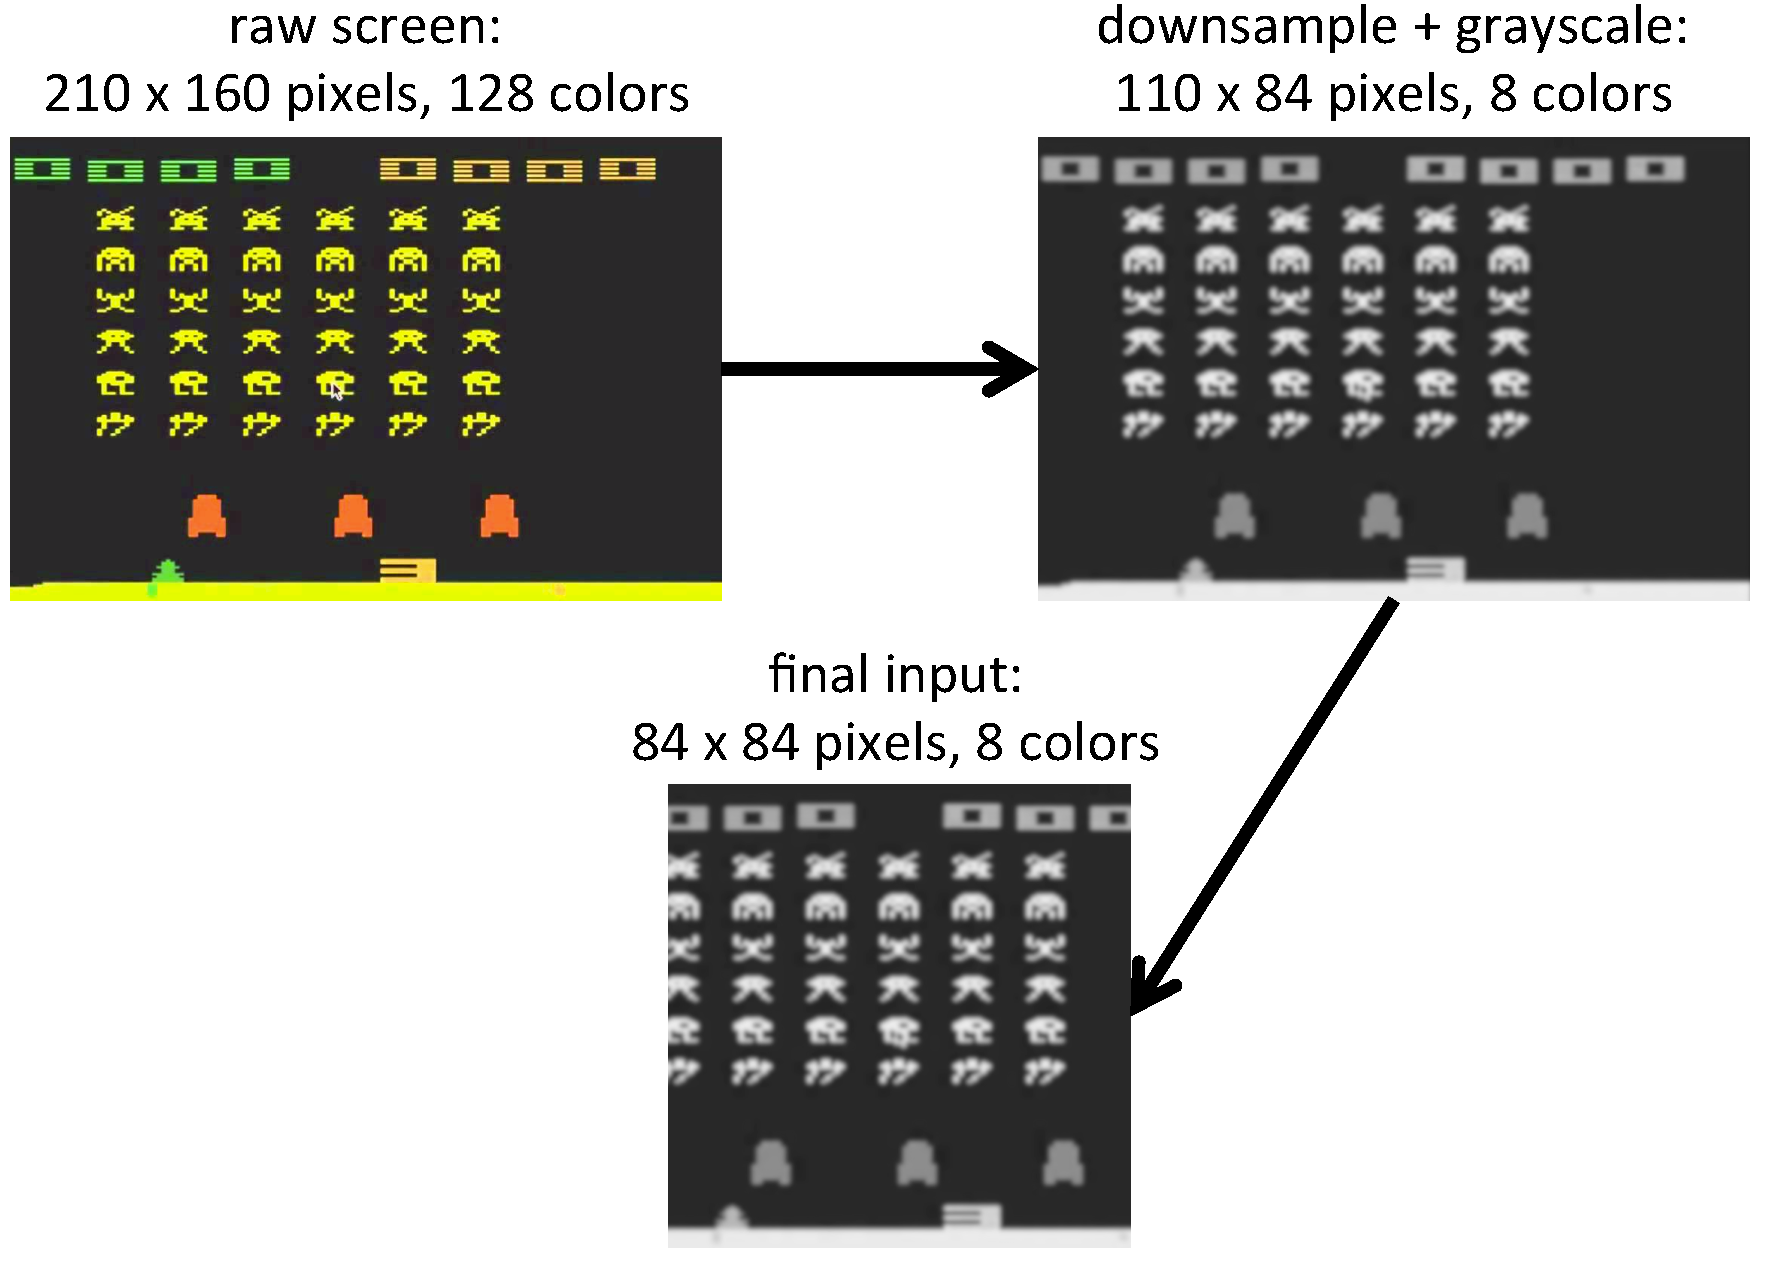
\includegraphics[width=0.9\textwidth]{process.pdf}
    \end{figure}
\end{frame}

\begin{frame}{Q-learning}
    \begin{itemize}\itemsep=12pt

        \item optimize Q-network loss function via
        \[
            Q\left(s,a\right) :=
            Q\left(s,a\right) +
            \alpha \left( r + \gamma\max_{a'}Q\left(s',a'\right) - Q\left(s,a\right) \right)
        \]
        
        \item trains optimal policy using ``behavior policy'' (off-policy)
        \vspace*{0.5em}
        \begin{itemize}
            \item learns policy $\pi^{\star}\left(s\right) = \argmax_{a}Q\left(s,a;\theta\right)$
            \item uses an $\epsilon$-greedy strategy (behavior policy) for state-space exploration
        \end{itemize}
    
    \end{itemize}
\end{frame}

\begin{frame}{Experience replay}
    a kind of short-term memory
    \vspace*{0.5em}
    \begin{itemize}\itemsep=12pt

        \item store agent's experiences at each time step
        \[
            e_{t} = \left(s_{t},a_{t},r_{t},s_{t+1}\right)
        \]
        
        \item experiences form a replay memory dataset
        \[
            \mathcal{D} = \left\{ e_{1}, \ldots, e_{N} \right\},
        \]
        where $N$ is the fixed memory capacity

        \item execute Q-learning updates with samples of experience
        \[
            e \sim \mathcal{D}
        \]

    \end{itemize}
\end{frame}

\begin{frame}{Serial deep Q-learning}
    \begin{tabbing}
        {\bf given} replay memory $\mathcal{D}$ with capacity $N$ \\*[\smallskipamount]
        {\bf initialize} Q-networks $Q$, $\hat{Q}$ with same random weights $\theta$ \\*[\smallskipamount]
        {\bf repeat} until timeout \\
            \qquad \= {\bf initialize} frame sequence $s_{1}=\left\{ x_{1} \right\}$ and preprocessed state $\phi_{1} = \phi\left(s_{1}\right)$ \\
            \> for \(t\) = 1, \(\ldots\) , \(T\) \\
            \qquad \qquad \= 1.\ select action $ a_{t} = \bigg\{
            \begin{tabular}{ll}
                $\max_{a}Q\left(\phi\left(s_{t}\right),a;\theta\right)$ & w.p. $1 - \epsilon$ \\
                \text{random action} & otherwise
            \end{tabular} $ \\
            \> 2.\ execute action $a_{t}$ and observe reward $r_{t}$ and frame $x_{t+1}$ \\
            \> 3.\ append $s_{t+1} = \left(s_{t}, a_{t}, x_{t+1}\right)$ and preprocess $\phi_{t+1} = \phi\left(s_{t+1}\right)$ \\
            \> 4.\ store experience $\left(\phi_{t},a_{t},r_{t},\phi_{t+1}\right)$ in $\mathcal{D}$ \\
            \> 5.\ uniformly sample minibatch $\left( \phi_{j},a_{j},r_{j},\phi_{j+1} \right) \sim \mathcal{D}$ \\
            \> 6.\ set $ y_{j} = \bigg\{
            \begin{tabular}{ll}
                $r_{j}$ & if $\phi_{j+1}$ terminal \\
                $r_{j} + \gamma\max_{a'}\hat{Q}\left(\phi_{j+1},a';\theta\right)$ & otherwise
            \end{tabular} $ \\
            \> 7.\ perform gradient descent step for $Q$ on minibatch \\
            \> 8.\ every C steps reset $\hat{Q} = Q$
    \end{tabbing}
\end{frame}

\section{Distributed algorithm}

\begin{frame}{Model parallelism}
    for each Q-network
    \vspace*{0.5em}
    \begin{itemize}\itemsep=12pt

        \item partition model across CPUs/GPUs
        \vspace*{0.5em}
        \begin{itemize}
            \item up to availability of CPU/GPU resources
            \item uses Caffe deep learning framework
        \end{itemize}

        \item \todo{Kevin/Hao Yi: How does caffe use CPU/GPU resources? How does complexity scale for implementation? Answers question of how our algorithm scale for model.}

    \end{itemize}
\end{frame}

\begin{frame}{Data parallelism}
    \textbf{downpour SGD:} generic asynchronous distributed SGD
    \begin{figure}
        \centering
        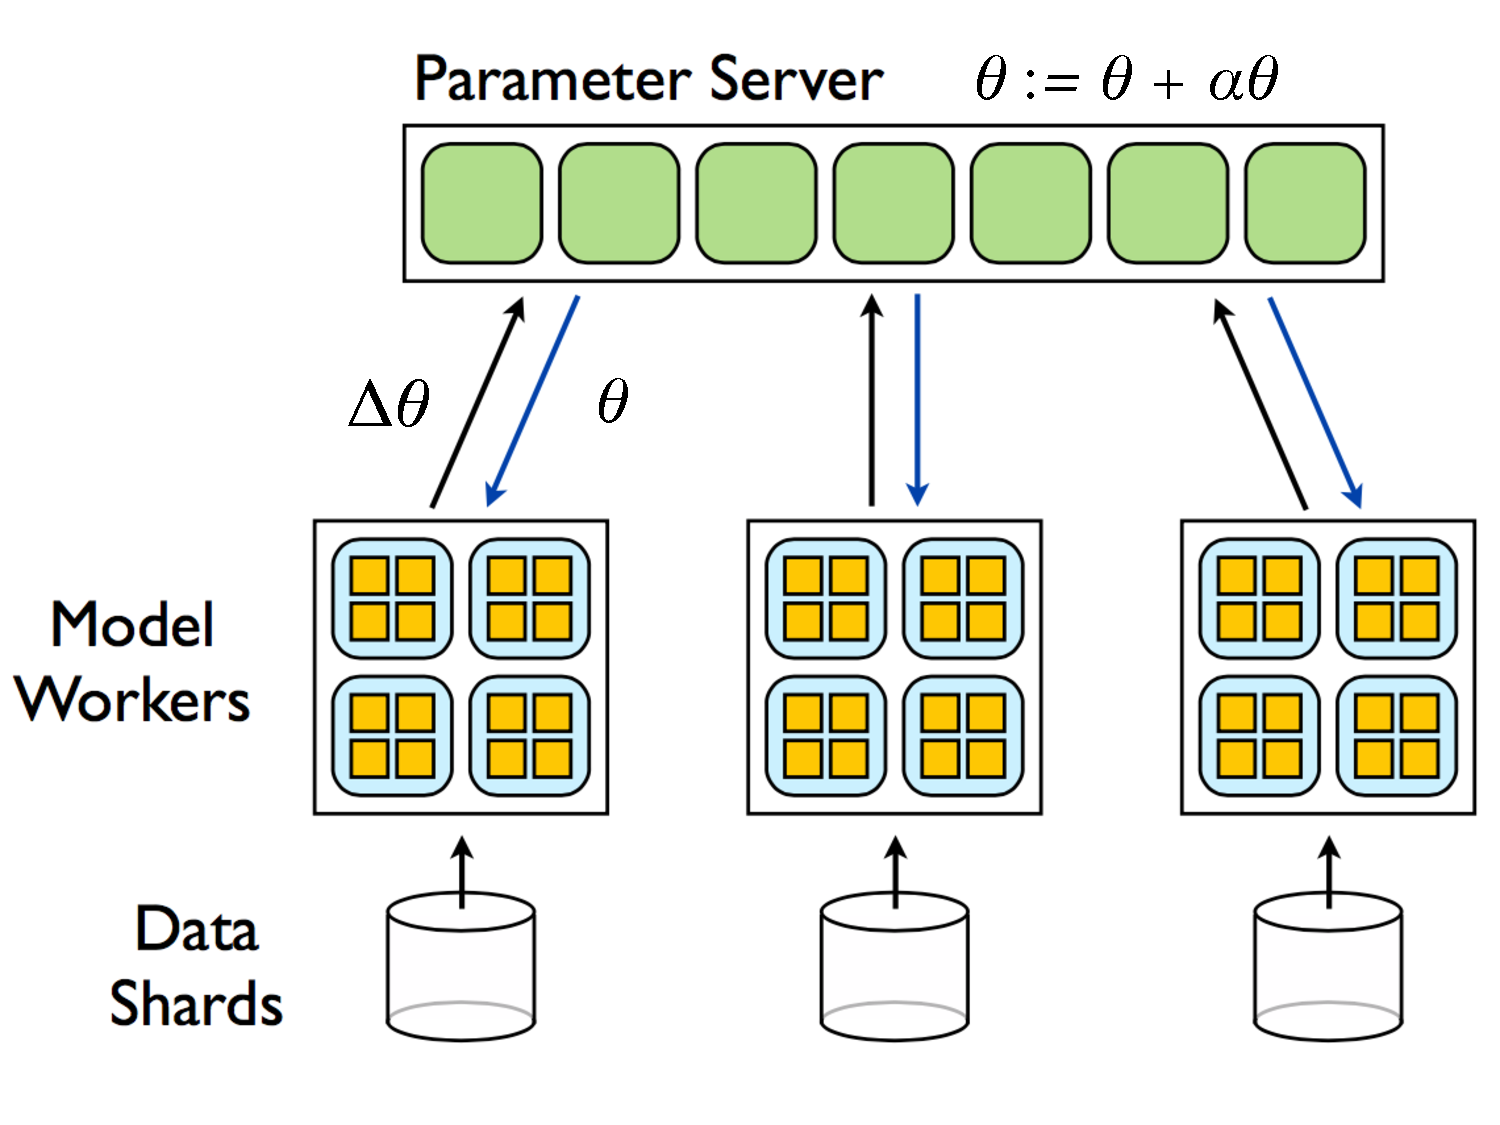
\includegraphics[width=0.8\textwidth]{data-par.pdf}
    \end{figure}
\end{frame}

\begin{frame}{Implementation}
    \begin{itemize}\itemsep=12pt

        \item data shards are generated locally on each model worker in real-time
        \vspace*{0.5em}
        \begin{itemize}
            \item data is stored independently for each worker
            \item since game emulation is simple, generating data is fast
            \item simple fault tolerance approach: regenerate data if worker dies
        \end{itemize}

        \item algorithm scales very well with data
        \vspace*{0.5em}
        \begin{itemize}
            \item since data lives locally on workers, no data is sent
        \end{itemize}

    \end{itemize}
\end{frame}

\begin{frame}{Implementation}
    \begin{itemize}\itemsep=12pt

        \item bottleneck is parameter update time on parameter server
        \vspace*{0.5em}
        \begin{itemize}
            \item \eg, if parameter server gradient update takes 2 ms, then we can only do up to 500 updates per second (using buffers, etc.)
        \end{itemize}

        \item trade-off between parallel updates and model staleness
        \vspace*{0.5em}
        \begin{itemize}
            \item because worker is likely using a stale model, the updates are ``noisy'' and not of the same quality as in serial implementation
        \end{itemize}

    \end{itemize}
\end{frame}

\begin{frame}{Implementation}
    communication pattern
    \vspace*{0.5em}
    \begin{itemize}\itemsep=12pt
        
        \item one-to-all and all-to-one, but asynchronous for every minibatch

        \item like multiple asynchronous all-reduces

    \end{itemize}
\end{frame}

\section{Numerical experiments}

\begin{frame}{Evaluation}
    \begin{figure}
        \centering
        
\includegraphics[height=0.6\textheight]{snake.png}
    \end{figure}
\end{frame}

\begin{frame}{Snake}
    \begin{itemize}\itemsep=12pt
        
        \item parameters
        \vspace*{0.5em}
        \begin{itemize}
            \item snake length grows with number of apples eaten
            \item one apple at any time, regenerated once eaten
            \item $n \times n$ array, with walled-off world
            \item want to maximize score, equal to snake length
        \end{itemize}

        \item complexity
        \vspace*{0.5em}
        \begin{itemize}
            \item four possible states for each cell: $\left\{ \mbox{empty, head, body, apple} \right\}$
            \item state space cardinality is $O\left(n^{8}\right)$
            \item four possible actions: $\left\{ \mbox{north, south, east, west} \right\}$
        \end{itemize}

    \end{itemize}
\end{frame}

\begin{frame}{Results}
    
\end{frame}

\section{Conclusion}

\begin{frame}{Summary}
    
\end{frame}

\section*{}

\begin{frame}[allowframebreaks]{References}
    \bibliography{IEEEabrv,slides}
\end{frame}

\section*{Appendix}

\begin{frame}{Theoretical complications}
    deep learning algorithms require
    \vspace*{0.5em}
    \begin{itemize}\itemsep=12pt

        \item huge training datasets

        \item independence between samples

        \item fixed underlying data distribution

    \end{itemize}
\end{frame}

\begin{frame}{Deep Q-learning}
    avoids theoretical complications
    \vspace*{0.5em}
    \begin{itemize}\itemsep=12pt

        \item greater data efficiency
        \vspace*{0.5em}
        \begin{itemize}
            \item each experience potentially used in many weight udpates
        \end{itemize}

        \item reduce correlations between samples
        \vspace*{0.5em}
        \begin{itemize}
            \item randomizing samples breaks correlations from consecutive samples
        \end{itemize}

        \item experience replay averages behavior distribution over states
        \vspace*{0.5em}
        \begin{itemize}
            \item smooths out learning
            \item avoids oscillations or divergence in gradient descent
        \end{itemize}

    \end{itemize}
\end{frame}

\end{document}